\chapter{Design of Cloud-SAP}

\chapterintro{ This chapter introduces the high-level design of Cloud-SAP.
  Further elaboration on the requirements of the proposed platform is presented
  and detailed discussion about the each its layer is held.
}

\section{Requirements}

\subsection{Functional}
One can notice that elements that yields a solution for
a problem stated in the first chapter, which is ensuring that users'
application provide appropriate Quality-of-Service for its customers, were
introduced in previous chapters:

\begin{itemize}
	\item scalability           -- ability to improve application performance by enriching
	\item adaptivity            -- ability to adapt (i.e. scale) appropriately to current usage pattern
	\item inter-cloud awareness -- ability to cooperate with different cloud provider to supply application with extra resources
\end{itemize}
Having those in mind, we can make the list of functional requirements more formal:
\begin{enumerate}
  \item The user of the platform is able to:
    \begin{enumerate}
      \item deploy a service,
      \item cancel the service,
      \item check the status of the previously ordered-to-deploy service at any time. \emph{Status} means 
        \begin{inparaenum}[a)]
        \item whether or not the deployment succeeded,
        \item current uptime of the service,
        \item current cost
        \end{inparaenum}
    \end{enumerate}
  \item One of the elements of the platform is a client application that is used by the user of the platform to communicate with it,
  \item During the deployment process, the platform takes as an input a description of the service (application) that consists of:
    \begin{itemize}
    \item service name,
    \item software stacks (e.g. \emph{java}, \emph{ruby}),
    \item auto-scaling policies (per each stack) which define
      \begin{inparaenum}[i)]
      \item minimal and maximal number of VMs that are needed for the stack,
      \item name of the policy (algorithm) which is used for scaling,
      \item parameters of the policy
      \end{inparaenum}
    \end{itemize}
  \item Deployment of a service is done in a way which minimizes the cost from the client's perspective with ensuring Quality-of-Service requirements at the same time,
  \item It is assumed that the application which is going to be deployed is properly and fully tuned so that it is not possible to improve its performance by changing its or any of its components configuration(s),
  \item The platform monitors the state of the deployed services and based on the results of this process takes appropriate steps in order to meet the auto-scaling requirements. These include
    \begin{inparaenum}[a)]
    \item altering VM's parameters and configuration,
    \item vertical scaling,
    \item horizontal scaling,
    \item scaling stacks among different cloud providers
    \end{inparaenum}
\end{enumerate}

TODO Alternative scenario -- the client has a predefined budget that they cannot exceed -- it can be mentioned in the overall discussion of the solution

\subsection{Non-functional}
\begin{itemize}
  \item The platform uses \emph{OpenVZ} as a hypervisor
  \item The platform uses \emph{OpenNebula} and \emph{OneApps} as data-center management tools
  \item The platform does not confine itself to one provider, but to a \emph{ecosystem of various cloud providers} that offers deployment capabilities which vary in terms of quality of service, cost, etc.
  \item All communication between the user and the platform and among platform components should be encrypted
\end{itemize}

\section{High-level design}
\subsection{Elements of the architecture}
In the previous chapters different scalability models were introduced where each operated at a different layer of abstraction: 
\begin{itemize}
	\item application platform tuning
	\item single-server level (vertical scaling)
	\item multi-server level (horizontal scaling) 
	\item inter-cloud level (scaling out across different cloud providers)
\end{itemize}

To reduce the system design complexity it is vital that proposed solution's
architecture reflects that multi-layered model. Thus, we divided platform's components into a stack that is shown in figure \ref{design:csap-layers}.

\begin{figure}[!ht]
  \begin{center}
    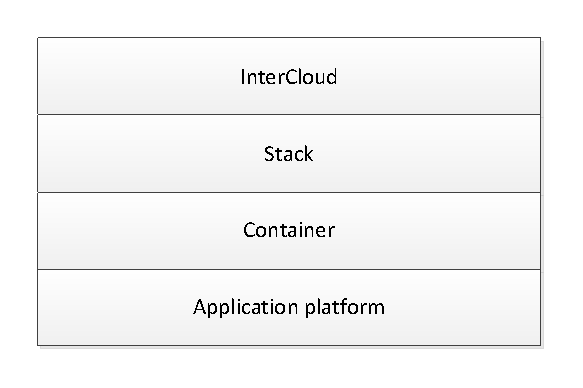
\includegraphics[width=0.5\textwidth]{chapter-5/sap-layers}
  \end{center}
  \caption{Layered structure of Cloud-SAP}
  \label{design:csap-layers}
\end{figure}

\subsection{Components autonomy}
Each layer of the Cloud-SAP (shown in figure \ref{design:csap-layers}) must be characterized by an ability to adapt to a given application usage. As the previous chapter stated, this can be achieved by adding an elasticity controller to each layer. This observation is a foundation of proposed architecture.

One of the first models that ensured system adaptivity is an autonomic component, concept based on a feed-back loop, initially proposed by IBM \cite{IBM06}. Figure \ref{ch5:autonomic-component} depicts that architecture. 

\begin{figure}[!ht]
  \begin{center}
    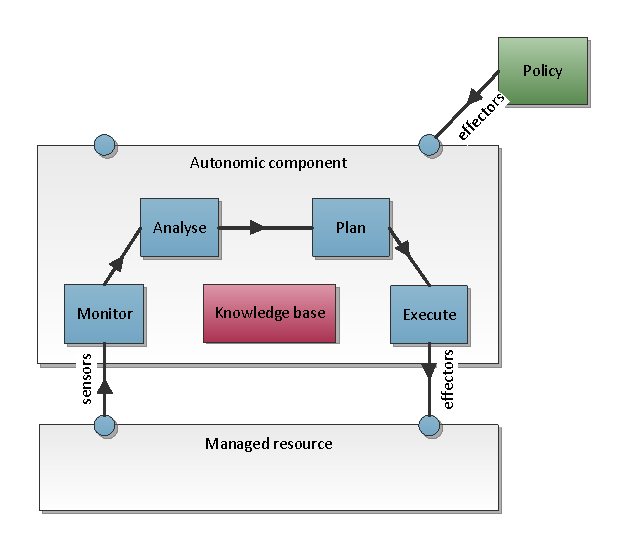
\includegraphics{chapter-5/autonomic-component}
  \end{center}
  \caption{autonomic component}
  \label{ch5:autonomic-component}
\end{figure}

Since designed platform operates on multiple layers, we can extend that model by using concept of a multi-hierarchical autonomic system \cite{LiWoZh05}. Figure \ref{ch5:hierarchical-autonomic-system} illustrates that hierarchy, were each level represents a different perspective at application scaling. Using terminology characteristic to a autonomic system, first three hierarchy levels (application tuning, single-server, multi-server) are centralized and controlled by single elasticity controller at each level, while the last inter-cloud level is a decentralized one - each cloud instance is fully independent.

\begin{figure}[!ht]
  \begin{center}
    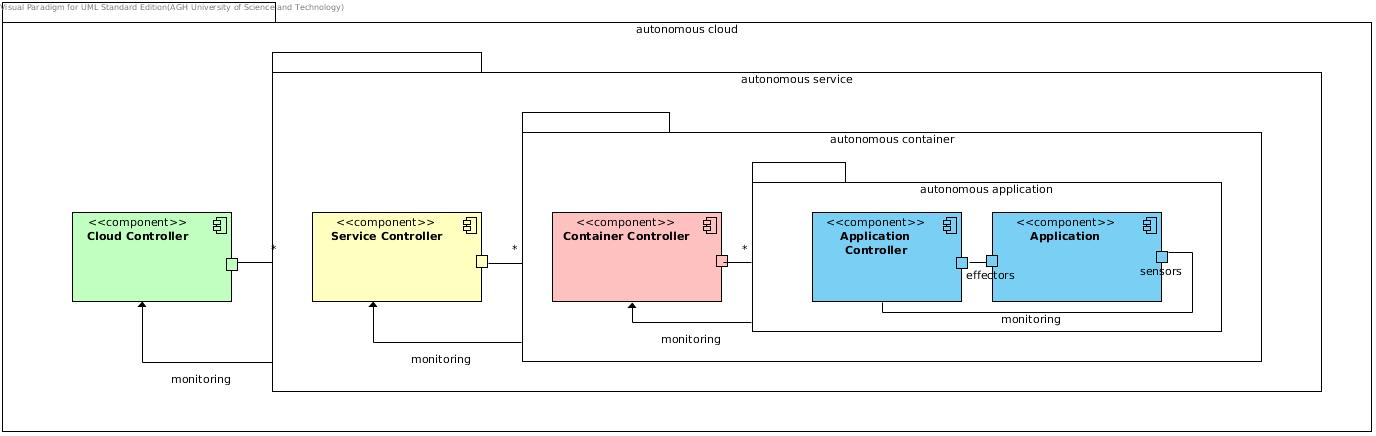
\includegraphics{chapter-5/hierarchical-autonomic-system}
  \end{center}
  \caption{Hierarchical autonomic system}
  \label{ch5:hierarchical-autonomic-system}
\end{figure}

As \cite{IBM06} states, each autonomic component has modules that are responsible for:
\begin{itemize}
	\item monitoring
	\item analysis
	\item planning
	\item action execution
\end{itemize}

While the managed component has:
\begin{itemize}
	\item sensors
	\item effectors
\end{itemize}

Due to the hierarchy of our architecture, each level manages an underlying autonomic component, while being managed by an upper layer at the same time. This lead us to observation that they are autonomic components and managed components at the same time. Remaining of this chapter discusses in detail each layer taking into account that observation.


